% Biểu mẫu D3 được đính kèm nguyên trạng. Xem ChuongTrinhThucTap.tex để biết lý do
% không dùng \section cho tiêu đề mục này.
% addtotoc tự tăng bộ đếm section và tự ghi số mục vào mục lục.
\IfFileExists{form/formD3.pdf}{
  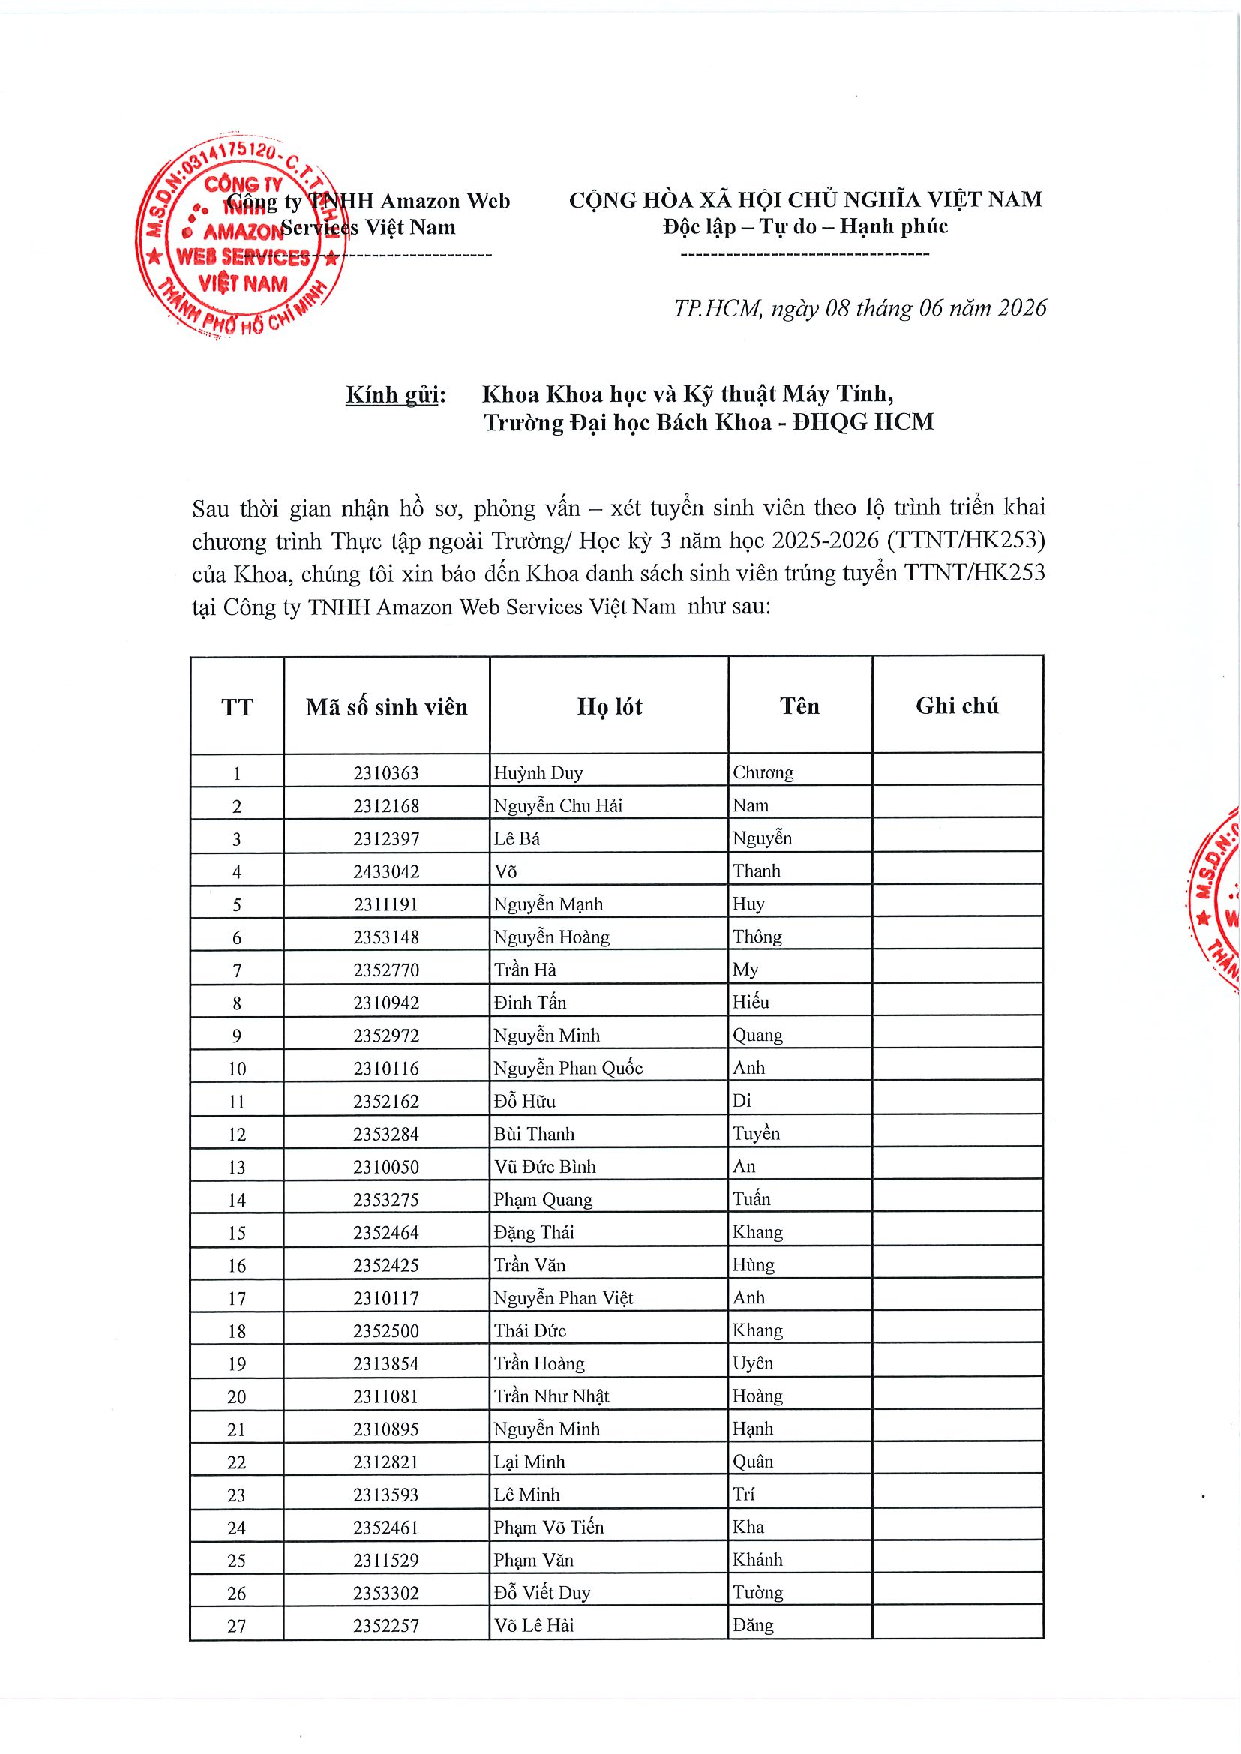
\includepdf[
    pages=-,
    addtotoc={1,section,1,Kết quả xét tuyển,sec:ket-qua-xet-tuyen},
    pagecommand={\thispagestyle{empty}}
  ]{form/formD3.pdf}
}{
    \refstepcounter{section}
    \phantomsection
    \addcontentsline{toc}{section}{\protect\numberline{\thesection}Kết quả xét tuyển}
    \begin{center}
        \textit{Đính kèm biểu mẫu D3 tại đây}
    \end{center}
    \pagebreak
}

\endinput
